\chapter{FHP}
This improved lattice gas cellular automaton is named after its inventors too -- Frisch, Humpfrey and Pomeu. 
They proposed it in 1986 together with its three dimensional variant - the FCHC. 
%Comparing it to HPP, we have a lattice with better rotational symmetry and nodes with richer  set of collisions.
%
Now that we presented the setting of FHP in two dimensions rather intuitively, let us explore the microdynamics of FHP in a more formal way. The formal treatment provides that the hydrodynamic equations that we derive are valid for FHP in arbitrary dimension (although finding an appropriate multidimensional lattice is non-trivial and possible only in 4 dimensions, as we will see).
In following section, we will graphically explain the basic principles of FHP, the other sections will be more general and the obtained results will be valid for arbitrary dimensional FHP-like automaton (most importantly FCHC).

\section{The lattice of FHP}
All the improvements of FHP are results of the simple change - instead of square grid, FHP builds on a hexagonal grid. 
%The two dimensional plane can be uniformly covered by squares, but also by hexagon, that . This is the main improvement of FHP, all other properties are implied by the properties of the hexagonal grid.

On the figure \ref{FHPgrid}, we have a part of the hexagonal grid, and from one of the nodes, six lattice vectors point to the neighboring nodes.
Let us denote the set of the lattice vectors by $c_i,~i=1,2,3,4,5,6$.


\begin{figure}[htbp] \label{FHPgrid}
 \centering
 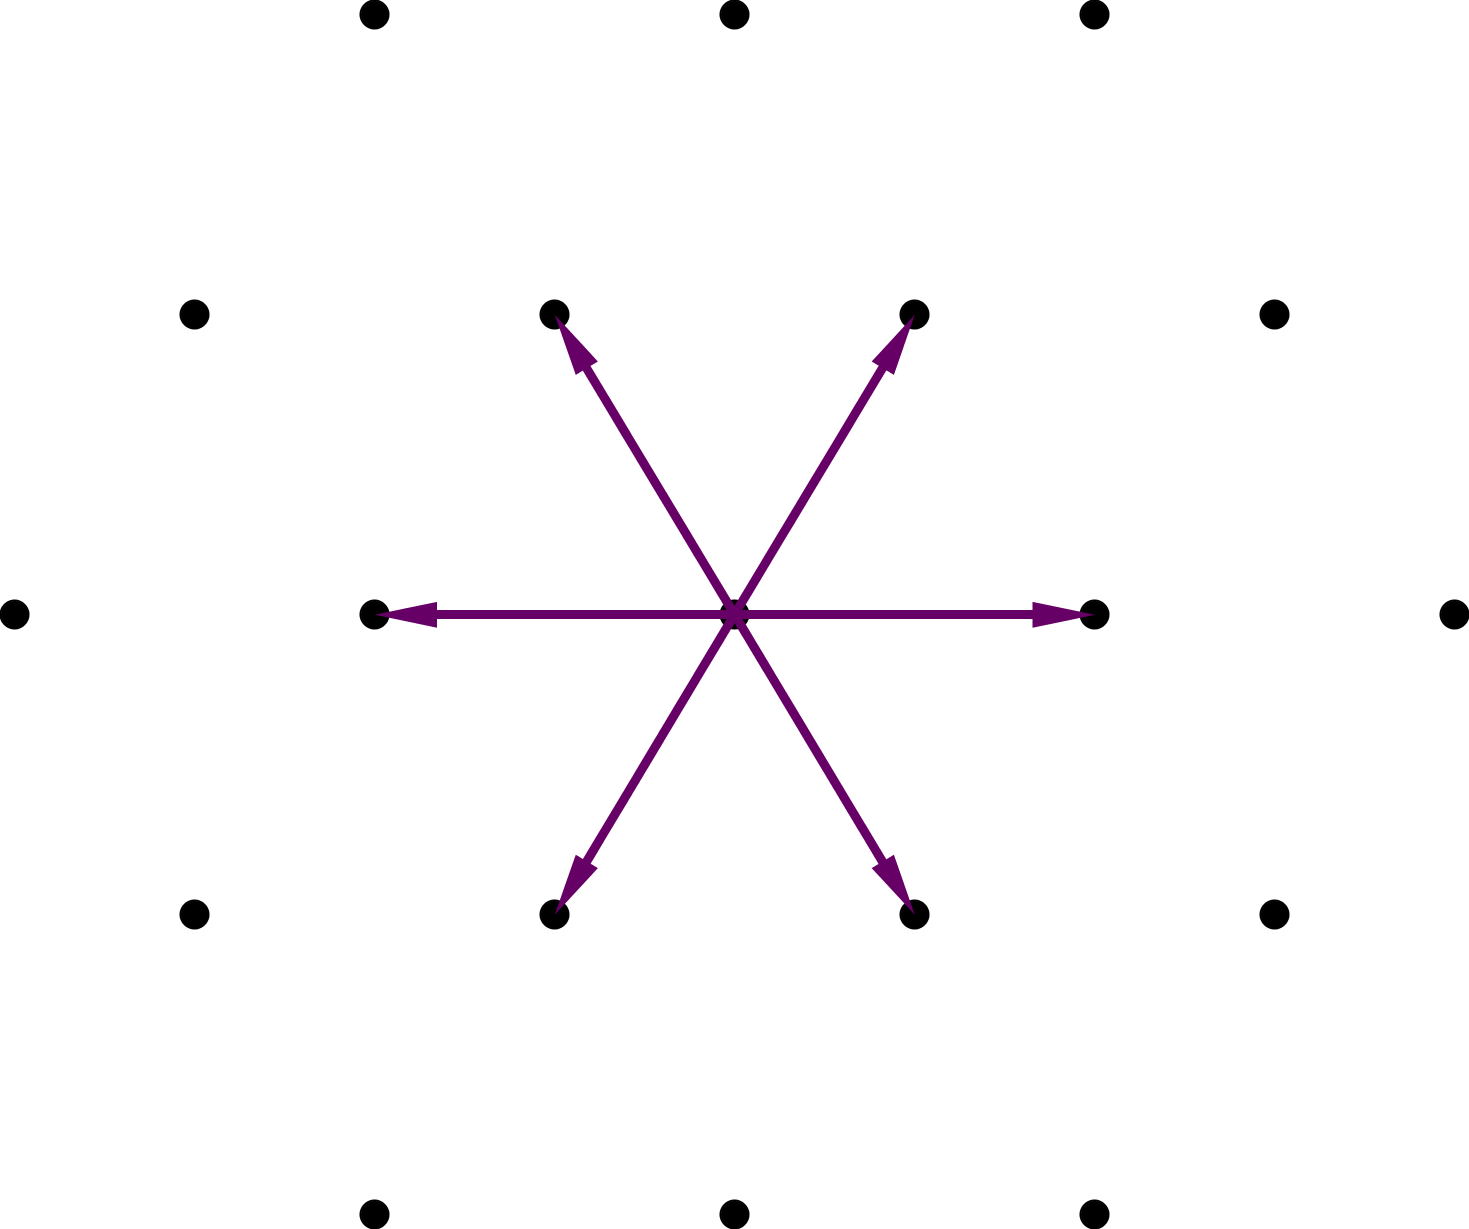
\includegraphics[width=0.6\textwidth]{./img/fhp_desc}
\end{figure}

The node is nothing else then a set of the six cells and each of the cells corresponds to one of the lattice vectors.
Let us denote the state of the node by $\bm{n} = (n_1,n_2,n_3,n_4,n_5,n_6)$, where $n_i = 0$ stands form empty $i^{th}$ cell, and $n_i = 1$ implies that there is a particle in the $i^{th}$ cell. 

State of a node with the position $\bf{r}$ on lattice will be denoted by $\bf{n(r)}$, whereas the state of the \textit{whole lattice} will be denoted by \textbf{n(.)}.

\section{Update rule}
As we know, the update happens in discrete time steps ($t=1,2,3...$) and consists of two subsequent steps - collision and propagation. Both of these steps are local, so they can be treated node by node.

\subsection{Propagation}

Propagation is the straight-forward phase and can be captured by the simple equation
\begin{align*}
S n_i(\bf{r}) = n_i(\bf{r + c_i}). 
\end{align*}
%This equation means that state of the $i^{th}$ cell in node \textbf{n(r)} \textit{propagates} along the lattice vector $c_i$ to the neighboring node $\bf{n(r + c_i)}$, the figure \ref{FHPprop}.
If the cell is occupied by a particle -- $n_i(\bf{r})=1$, it propagates along the corresponding lattice vector to the neighboring node, see the figure \ref{FHPprop}.

\begin{figure}[H]
 \centering
 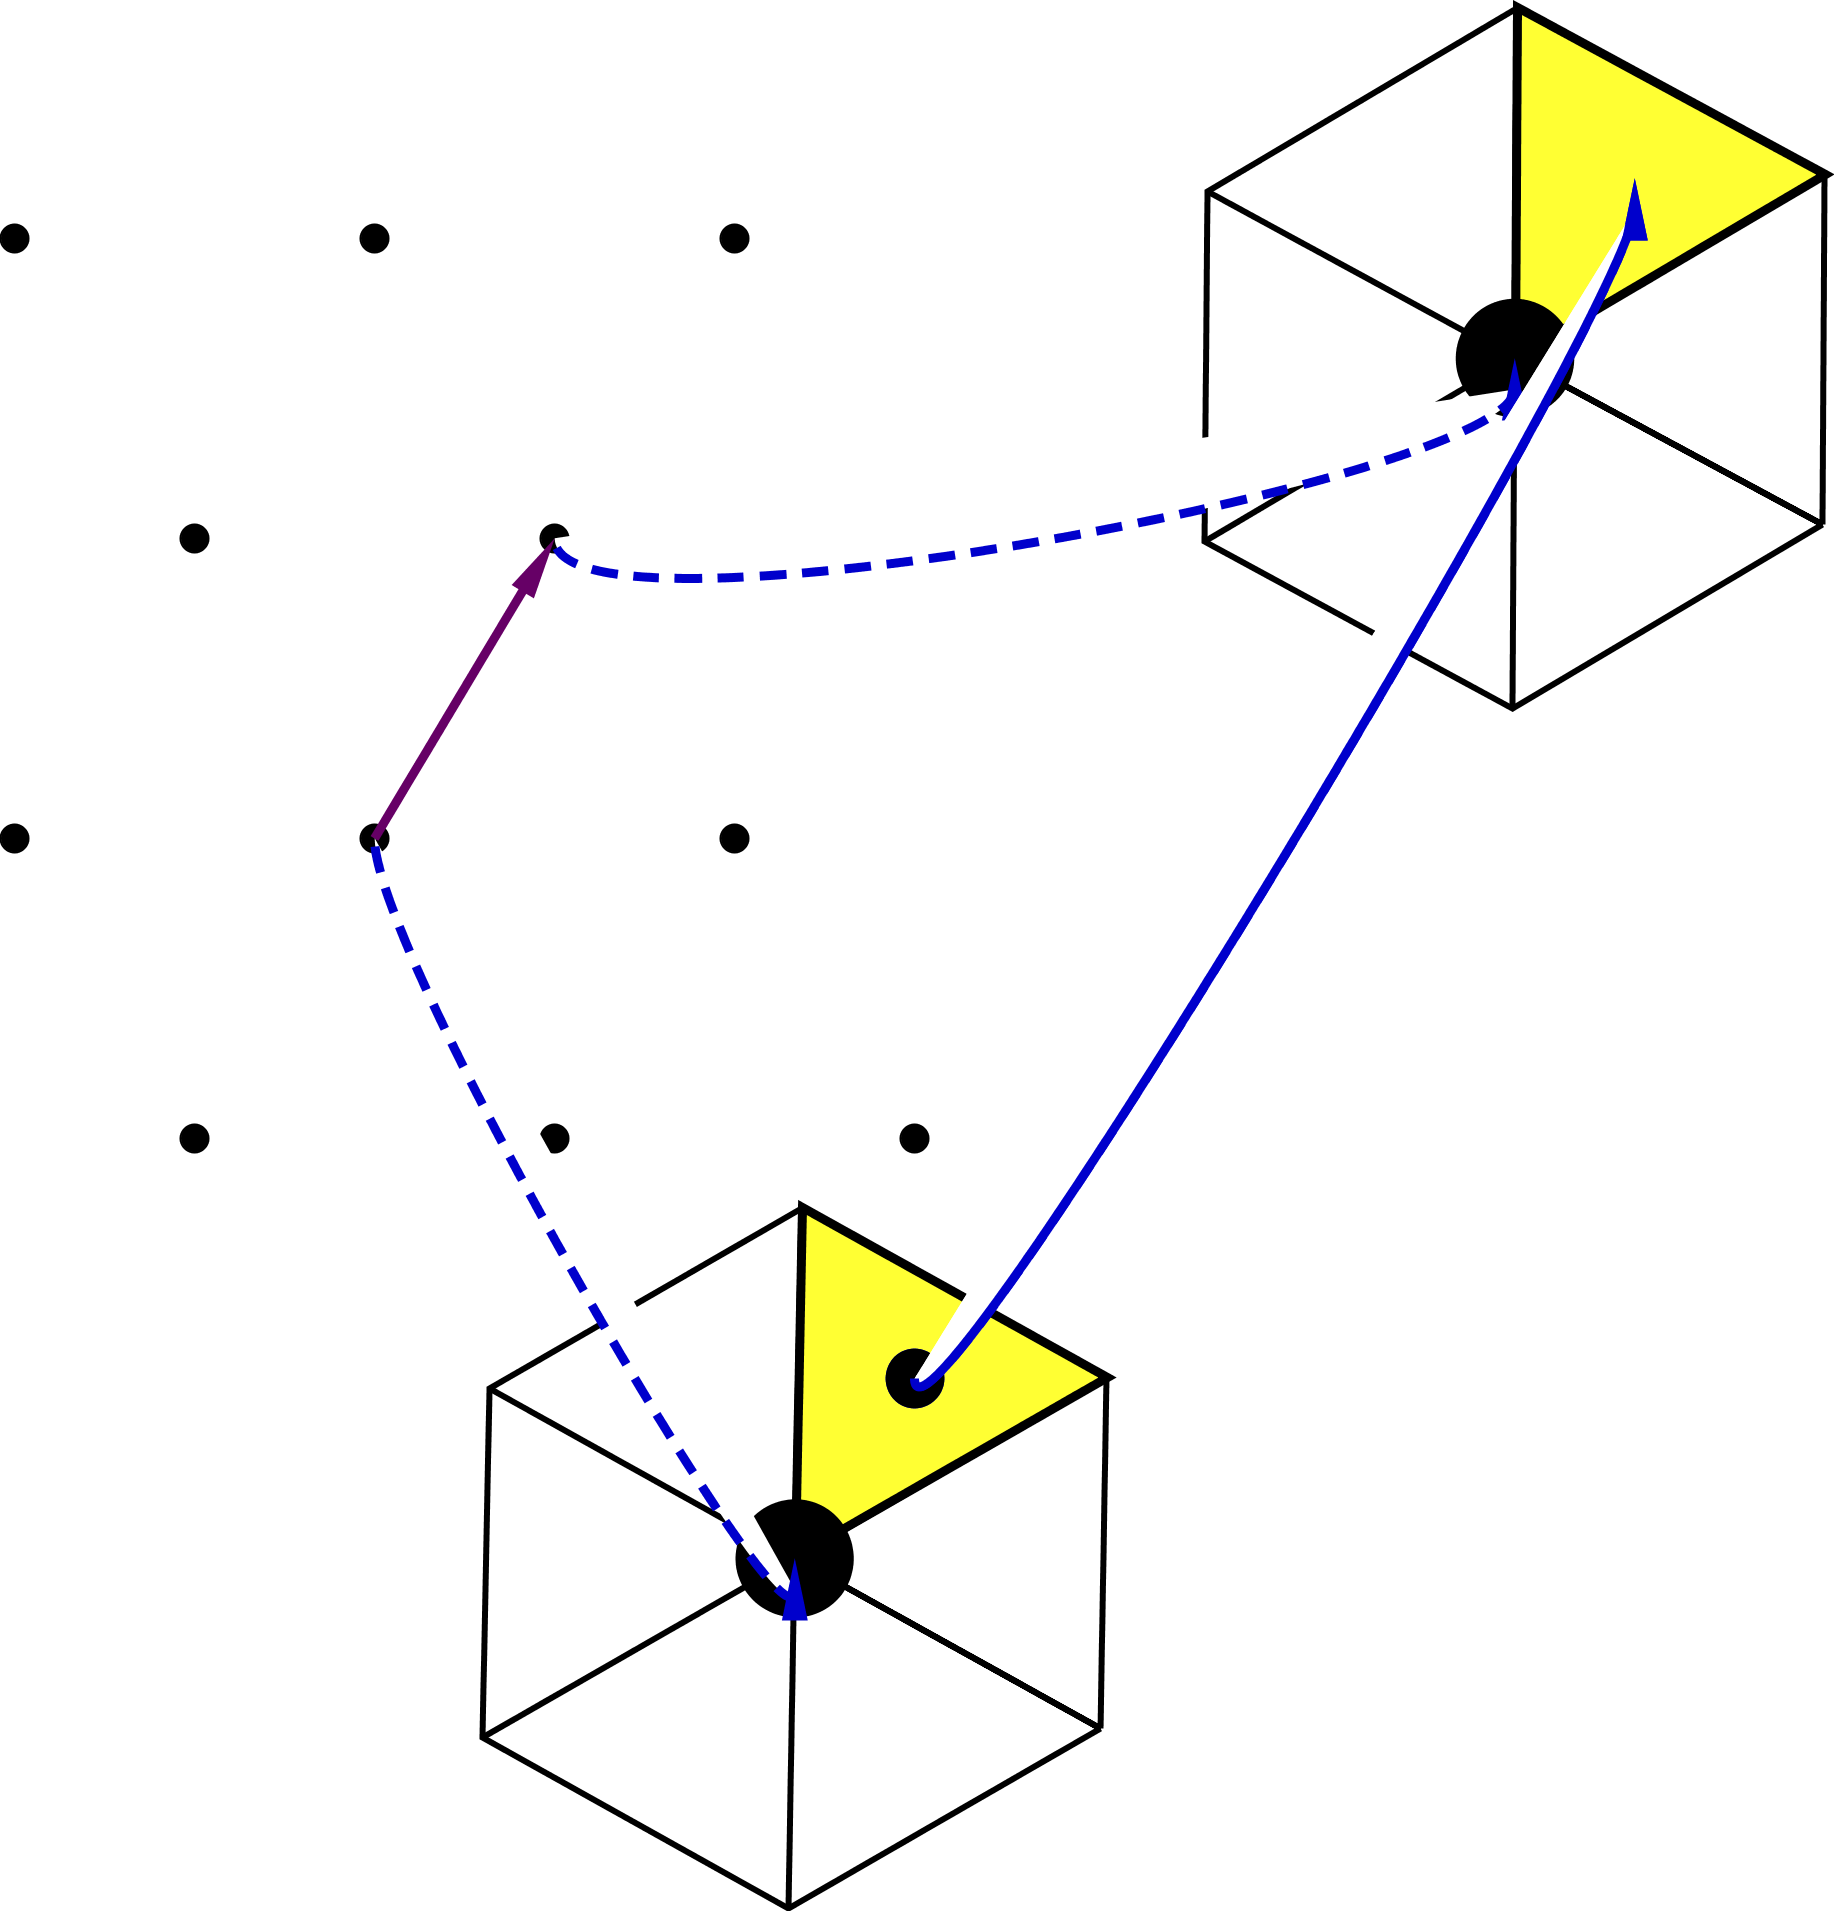
\includegraphics[width=0.7\textwidth]{./img/FHPprop}
 \caption{FHP collisions without rest particle.}
 \label{FHPprop}
\end{figure}
The propagation, however, is preceded by the more interesting step -- the collision.

\subsection{Collision}

The purpose of the collision is to swap as many particles in the node as possible.
The only constraint on the collision rule is to preserve the number of particles (conservation of the mass) and to preserve the total momentum in the node.

These requirements lead only to a handful of collision configurations, see figure \ref{FHPcol}. For the simplicity, we are considering the FHP-I model, that does not included the "rest particles", otherwise we would have few more rules to add.

\begin{figure}[H]
 \centering
 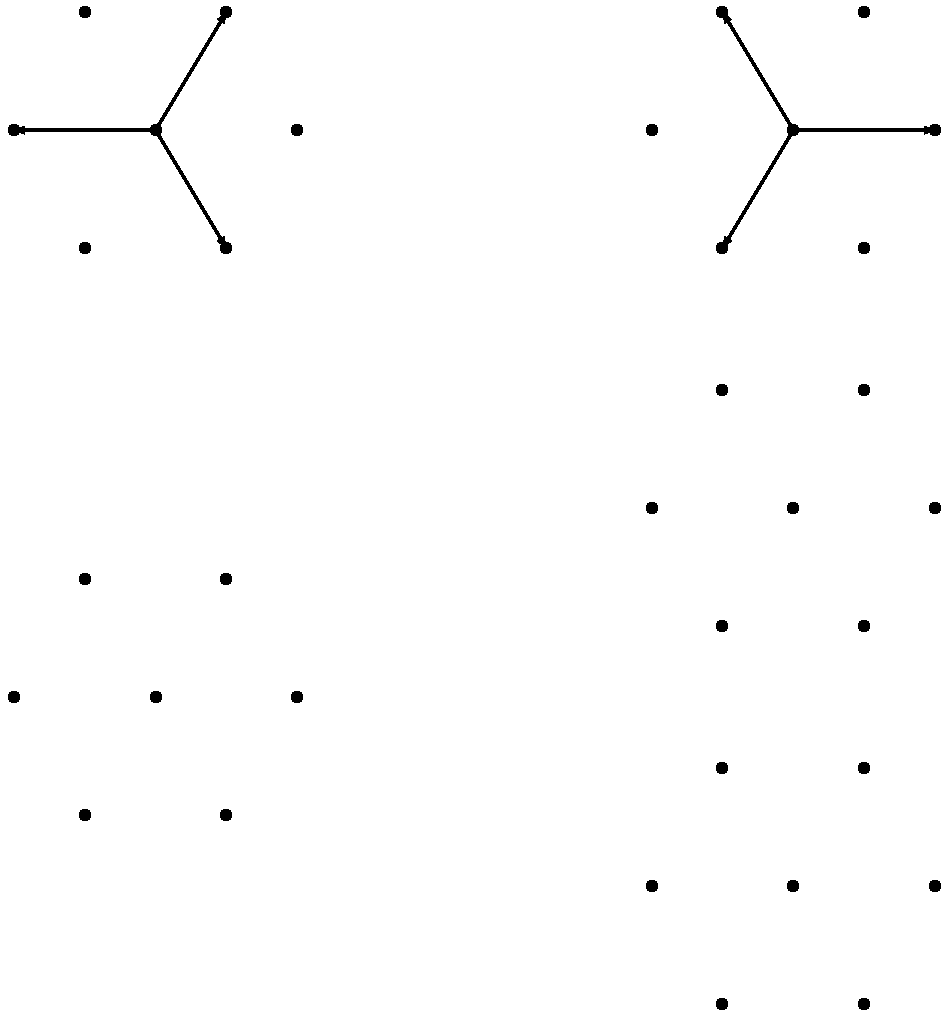
\includegraphics[width=0.7\textwidth]{./img/FHPcol}
 \caption{FHP collisions without rest particle.}
 \label{FHPcol}
\end{figure}

We see that two and four particle configurations can be resolved in two different configurations. The resulting state need to be chosen randomly, with probability $1/2$ for each state to preserve the parity symmetry of the model. If we were systematically choosing only one of them, we would introduce additional, non-physical invariant - chirality. Hence, we need to introduce non-determinism to the model.


We will express the probabilities of transition from state $n$ to state $n'$ by probability matrix:
\begin{align*}
A(n \rightarrow n') \geq 0
\end{align*}
As we have 64 possible states of the node, matrix A is of dimension $64\times 64$.
For example, the cell of matrix A that governs the head-on collisions looks like this:
\[
 A'=
  \begin{bmatrix}
    0 & \frac{1}{2} & \frac{1}{2} \\
    \frac{1}{2} & 0 & \frac{1}{2} \\
    \frac{1}{2} & \frac{1}{2} & 0 \\
  \end{bmatrix}
\]
Since the collisions are symmetric, matrix A is symmetric as well.

Also, collisions are invariant to rotations and reflections of the node:
\begin{align*}
A(g(n) \rightarrow g(n')) = A(n \rightarrow n')
\end{align*}
where $g \in G$, and G is the symmetry group of the node.


\section{Collision operator}
Interestingly, we can express the whole update step in one simple equation using collision operator $\Delta_i$:
\begin{align} \label{withcol}
n_i(t+1,r+c_i) = n_i(t,r) + \Delta_i(t,r)
\end{align}
where $\Delta_i$ is
\begin{enumerate}
\item $\Delta_i = 0$ if no collision is happening in $n(t,r)$. Then state of the cell $n_i(t,r)$ only propagates to $n_i(t+1,r+c_i)$.
\item $\Delta_i = 1$ if there is not particle in $n_i(t,r)$ yet, but gets there after collision. 
\item $\Delta_i = -1$ if there is particle in the $n_i(t,r)$, but after collision, cell gets empty.
\end{enumerate}

\bigskip

%For example, $\Delta_i$ acquire very simple form for HPP
%\begin{equation*}
%\Delta_i = n_{i+1} n_{i+3}( 1 - n_i)(1 - n_{i+2}) - n_i n_{i+2}(1-n_{i+1})(1 - n_{i+3}).
%\end{equation*}
%As there are only 2 collision configuration in HPP, $\Delta_i$ has 2 terms.

By this reasoning, we obtain the form of collision operator for FHP-I model
\begin{align} \label{colop}
\begin{split}
\Delta_i = n_{i+1}n_{i+3}n_{i+5}(1-n_i)(1-n_{i+2})(1-n_{i+4})\\
-n_in_{i+2}n_{i+4}(1-n_{i+1})(1-n_{i+3})(1-n_{i+5})\\
 + \xi n_{i+1}n_{i+4}(1-n_i)(1-n_{i+2})(1-n_{i+3})(1-n_{i+5})\\
 +(1-\xi)n_{i+2}n_{i+5}(1-n_i)(1-n_{i+1})(1-n_{i+3})(1-n_{i+4})\\
 -n_in_{i+3}(1-n_{i+1})(1-n_{i+2})(1-n_{i+4})(1-n_{i+5}).
\end{split}
\end{align}

\section{Microscopic conservation laws}
We can easily prove that
%By substituting \ref{colop} for the collision operator, we can prove that
\begin{align*}
\begin{split}
\sum_i \Delta_i(t,r) &= 0,\\
\sum_i c_i \Delta_i(t,r) &= 0.
\end{split}
\end{align*}
by substituting \ref{colop} into these equations. Combining with \ref{withcol}, they imply the simple form for the conservation of mass and momentum
%Therefore, the laws of mass and momentum conservation acquire the simple form
\begin{align} \label{cons1}
\begin{split}
\sum_i n_i(t+1, r + c_i) &= \sum_i n_i(t,r), \\
\sum_i c_i n_i(t+1, r + c_i) &= \sum_i c_i n_i(t,r).
\end{split}
\end{align}
By employing the aparatus of the statistical physics we will show that these microscopic conservation laws lead to physically realistic macroscopic description.

\section{Conservation of probabilities}
Let us define the phase space $\Gamma$ as the set of all possible states of the lattice $n(.)$.
Imagine we want to initialize cellular automaton with some macroscopic velocity $\bm{v_0}$, macroscopic pressure $p_0$, and macroscopic density $\rho_0$.
We can realize this macrostate by very many microstates of lattice $n(.)$.
We assign initial probability to each of these microstates:
\begin{align*}
P(0,s(.)) \geq 0.
\end{align*}
Of course, probabilities over whole lattice are normalized so
$\sum_s(.) P(0,s(.)) = 1$.

In the statistical mechanics, Liouville's space state theorem postulates that the density of the phase space is constant. Microdynamics of our model implies equivalent theorem for LGCA:
\begin{align*}
P(t+1, \mathcal{E} s(.)) = P(t, s(.))
\end{align*}

It is obtained directly by applying the update formula
\begin{equation*}
\mathcal{E} s(t,.) = s(t+1,.)
\end{equation*}
However, for indeterministic model such as FHP, the conservation of probability is governed by the more general formula
\begin{equation}
P(t+1,\mathcal{S} n'(.)) = \sum_{n(.) \in \Gamma} \prod_{n(.)} A(n(\bm{r} \rightarrow n'(\bm{r})) P(t, n(.)),
\end{equation}
that constitutes the LGCA version of Chapman-Kolmogorov equation.

\section{Mean occupation numbers}
Motivated by the ensemble formalism of statistical physics, we define mean occupation numbers
\begin{equation*}
N_i = \langle n_i \rangle = \sum_{s(.) \in \Gamma} n(s(.)) P(t,s(.)) .n
\end{equation*}

This formula naturally suggests definition of the mean mass density
\begin{equation*}
\rho(t,r) = \sum_i N_i(t,r)
\end{equation*}
and the momentum density
\begin{equation*}
j(t,r) = \sum_i c_i N_i
\end{equation*}

Due to conservation of probabilities, the conservation laws \ref{cons1} implies conservation of the mean quantities
\begin{equation} \label{macro1}
\sum_i N_i(t+1,r+c_i) = \sum_i N_i(t,r) 
\end{equation}
\begin{equation} \label{macro2}
\sum_i c_i N_i(t+1,r+c_i) = \sum_i c_i N_i(t,r)
\end{equation}

\section{Equilibrium occupation numbers}
After laborious definitions in previous sections, we are ready for one of the central theorems for FHP. It states that the equilibrium occupation numbers are given by Fermi-Dirac distribution. Its implications will haunt us until the last chapter.

We state it without the lengthy proof, but we recommend \cite{wolf} or \cite{frisch} for the non-believers.

\bigskip
Since the formalism that we were using in previous section is independent of the dimension of FHP, we can state this theorem for the FHP-like automaton in arbitrary dimension $D$ with the lattice vectors $c_i \in R^D,~i=1...b$.

\bigskip

\textbf{Theorem 1:}
The following statements are equivalent:
\begin{enumerate}
\item $N_i^{eq}$s are solutions of Chapman-Kolmogorov equation (reference)\\
\item $N_i^{eq}$s are solutions of set of b equations:
\begin{equation}
\Delta_i(N) = \sum_{nn'}(n'_i - n_i)A(n \rightarrow n')\prod_j N_j^{n_j}(1-N_j)^{1-n_j}
\end{equation} 

\item $N_i$ are given by Fermi-Dirac distribution
%\begin{align} \label{fd}
%N_i^{eq} = \frac{1}{1 + \exp(h + \bm{q}.\bm{c_i})},
%\end{align}
where h is real number and \textbf{q} is D-dimensional vector.
\end{enumerate}

\bigskip

To express $N_i^{eq}$ explicitly as function of $\rho$ and $\bm{u}$, we employ technique of Lagrange multipliers with natural constraints
\begin{equation}
\rho = \sum_i N_i = \sum_i \frac{1}{1+ exp(h + \bm{q}.\bm{c_i})}
\end{equation}
\begin{equation}
\bm{u} = \sum_i \bm{c_i} \bm{N_i} = \sum_i \frac{\bm{c_i}}{1+ exp(h + \bm{q}.\bm{c_i})}
\end{equation}

Explicit solutions are available only in few special cases.
In general, we may use expansion for small Mach numbers ($\bm{u}/c_{\mathrm{sound}}$). By expansion up to second order, equilibrium distribution for $D$-dimensional FHP-like automaton reads \footnote{The expansion is required up to the second order, because the non-linear term in Navier-Stokes equations will emerge from the quadratic term}
\begin{equation} \label{eou}
N_i^{eq}(\rho,\bm{u}) = \frac{\rho}{b} + \frac{D\rho}{c^2 b}\bm{c_i}.\bm{u} = \rho G(\rho) Q_{i\alpha\beta}u_{\alpha}u_{\beta} + O(u^3)
\end{equation}
where 
\begin{align}
Q_{i\alpha\beta} = c_{i\alpha} c_{i\beta} - \frac{c^2}{D} \delta_{\alpha\beta}
\end{align}
and
\begin{align}
G(\rho) = \frac{D^2}{2c^4b}\frac{b-2\rho}{b-\rho}.
\end{align}

%Realizing that
%\begin{equation}
%\sum_i c_{i\alpha} c_{i\beta} = 
%\end{equation}

\section{Chapman-Enskog expansion}
Because relaxation towards equilibrium values happens in a few updates of the automaton, it is standard procedure to expand the occupation numbers $N_i(t,r)$ around the equilibrium occupation numbers $N_i^{eq}(\rho,\bm{u})$:
\begin{equation} \label{chap}
N_i(t,r) = N_i^0(t,r) + \epsilon N_i^1(t,r) + \mathcal{O}(\epsilon^2) 
\end{equation} 
%Following formulas
%\begin{equation}
%\rho = \sum_i N_i(t,r) = \sum_i N_i^{eq}(\rho,\bm{u})
%\end{equation}
%\begin{equation}
%\bm{j} = \sum_i c_i N_i(t,r) = \sum_i c_i N_i^{eq}(\rho,\bm{u})
%\end{equation}
%imply that


The equations of mass and momentum conservation \ref{macro1} and \ref{macro2} can be equivalently stated in the form
\begin{equation} \label{macro_m}
\sum_i N_i(t+1,r+c_i) - N_i(t,r) = 0 ,
\end{equation}
\begin{equation} \label{macro_p}
\sum_i c_i (N_i(t+1,r+c_i) - N_i(t,r)) = 0,
\end{equation}
that is more suitable for our purpose.

Expansion of $N_i(t+1,r+c_i)$ around $N_i(t,r)$ leads to
\begin{equation} \label{rozvoj t+1}
\begin{split}
N_i(t+1,r+c_i) = N_i(t,r) + \partial_t N_i(t,r) + c_{i\alpha} \partial_{\alpha} N_i(t,r) \\ 
+ \frac{1}{2} \partial_t \partial_t N_i(t,r) + \frac{1}{2} c_{i\alpha}c_{i\beta} \partial_{\alpha} \partial_{\beta} N_i(t,r) + c_{i\alpha} \partial_t \partial_{\alpha} N_i(t,r) + \mathcal{O}(\partial^3).
\end{split}
\end{equation}
\bigskip
The expression above is the mixture of various physical phenomena -- diffusion, advection, propagation of the sound waves or relaxation towards local equilibria. Each phenomena has its typical spatial and temporal scale, that corresponds to different powers of $\epsilon$, see the tables below. %\ref{scalings}.

\begin{center} 
    \begin{tabular}{| l | l | l | l |}
    \hline
    \multicolumn{3}{|c|}{ \label{scalings} TEMPORAL SCALES}\\ \hline
    \textbf{Scale} & \textbf{Rescaling of time} & \textbf{Phenomena} \\ \hline
    1 step & t & Relaxation towards local equilibrium \\ \hline
    100 steps & $t_1 = \frac{1}{100} t = \epsilon t$ & advection, sound waves (perturbation of mass and density) \\ \hline
    10 000 steps & $t_2 = \frac{1}{10000} t = \epsilon^2 t$ & diffusion \\ \hline
    \label{scalings}
    \end{tabular}
\end{center}


\begin{center}
    \begin{tabular}{| l | l | l | l |}
    \hline
    \multicolumn{3}{|c|}{SPATIAL SCALES}\\ \hline
    \textbf{Scale} & \textbf{Rescaling of length} & \textbf{Phenomena} \\ \hline
    1 lattice unit & \textbf{r} & Relaxation towards local equilibrium \\ \hline
    100 lattice units & $\bm{r_1} = \frac{1}{100} \bm{r} = \epsilon \bm{r}$ & diffusion, advection, sound waves\\ \hline
    \end{tabular}
\end{center}

To derive the hydrodynamical equation that we long for, we will exploit the multi-scale technique. It starts by grouping-up the terms of hydrodynamical temporal and spatial scales.


\bigskip
Using to rescaled the length and time, we deduce the rescaled differential operators
\begin{equation} \label{oper}
\begin{split}
\partial_t = \epsilon \partial_t^{(1)} + \epsilon^2 \partial_t^{(2)} \\
\partial_{\alpha} = \epsilon \partial_{\alpha}^{(1)}
\end{split}
\end{equation}

Now, we are ready to expand the conservation laws \ref{macro_m} and \ref{macro_p} by Chapman-Enskog. We insert expansion \ref{rozvoj t+1} of $N_i(t+1,r+c_i)$, then we insert expansion of $N_i(t,r)$ according to \ref{chap}. Finally, we substitute differential operators according to \ref{oper}.

We do not present the whole monstrous expansion, only the terms of order $\epsilon$, that we are interested in.

From conservation of mass \ref{macro_m} we get
\begin{equation}
\partial_t^{(1)} \sum_i N_i^{(0)} + \partial_{\beta} \sum_i c_{i\beta} N_i^{(0)} = 0,
\end{equation}
and from conservation of momentum \ref{macro_p} we get
\begin{equation}
\partial_t^{(1)} \sum_i c_{i\alpha} N_i^{(0)} + \partial_{\beta} \sum_i c_{i\alpha} c_{i\beta} N_i^{(0)} = 0.
\end{equation}

Using definition of mass density, and the following definition of the \textit{momentum flux tensor}
\begin{equation}
P^{(0)}_{\alpha\beta} := \sum_i c_{i\alpha} c_{i\beta} N_i^{(0)} = \sum_i c_{i\alpha} c_{i\beta} N_i^{eq}(\rho, \bm{u}).
\end{equation}
we can write the conservation laws in the shorter form
\begin{equation} 
\begin{split}
\partial_t^{(1)} \rho + \nabla^{(1)}(\rho \bm{u}) = 0, \\ 
\partial_t^{(1)} (\rho u_{\alpha}) + \nabla^{(1)} P^{(0)}_{\alpha\beta} = 0 \label{eul_primitive}
\end{split}
\end{equation}

In the first equation, we recognize the famous continuity equation, but we have some work to do with the second equation.

%Now is the time to observe, that:
%\begin{equation} \label{2mom}
%\sum_i c_{i\alpha}c_{i\beta} = 3\delta_{\alpha\beta}
%\end{equation}
%Using this observation and inserting formula for equilibrium occupation number \ref{eou} we can write:
%\begin{equation}
%P^{(0)}_{\alpha\beta} = \frac{\rho}{2} \delta_{\alpha\beta} 
%+ \rho G(\rho) \sum_i c_{i\alpha}c_{i\beta} Q_{i\gamma\delta} u_{\gamma} u_{\delta} + \mathcal{O}(u^4)
%\end{equation} 
Substituting \ref{eou} for $N_i^{eq}$ into momentum flux tensor, its components read (after some algebraic simplification)
\begin{equation} \label{FHPT}
\begin{split}
P_{xx}^{(0)} = \frac{\rho}{2}g(\rho)(u_x^2 - u_y^2) + \frac{\rho}{2},\\
P_{yy}^{(0)} = \frac{\rho}{2}g(\rho) (u_x^2 - u_y^2) + \frac{\rho}{2},\\
P_{xy}^{(0)} = P_{yx}^{(0)} = \rho g(\rho)u_xu_y,
\end{split}
\end{equation}
where we defined $g(\rho) =  \frac{3-\rho}{6 - \rho}$.

Unfortunately, it does not match the momentum flux tensor of Navier-Stokes equation
\begin{equation} \label{NST}
\begin{split}
P_{xx} = \rho \, u_x^2 + p\\
P_{yy} = \rho\, u_y^2 + p\\
P_{xy} = P_{yx} = \rho u_x u_y
\end{split}
\end{equation}

Let us examine why are these tensors different.

For low values of $\bm{u}^2$, pressure $p$ is given by isothermal relation \cite{wol} $p = \frac{\rho}{2} = \rho c_s^2$, where $c_s = \frac{1}{\sqrt{2}}$ is the speed of sound.

What about $g(\rho)$?  

The disease of FHP, FCHC and all lattice-gas cellular automata to follow is, that $g(\rho)$ is never equal to 1, as it is in Navier-Stokes equations.

The reason lies in the broken \textit{Galilei invariance} of LGCA,as they all have discrete rotational symmetry (by $60 \degree$ in FHP and between $60 \degree$ and $45 \degree$ in FCHC).

In the final chapter on theory of LGCA, we will show the fundamental treatment of this flaw. Symptomatic treatment, such as rescaling the time
\begin{align} \label{frac_resc}
t \rightarrow \frac{t}{g(\rho)},
\end{align}
does not solve all the associated problems (D'Humier et al. 1987).

However, using this rescaled time, and setting density to be constant ($\rho = \rho_0$ except for the pressure term \ref{press}), we get the familiar incompressible Euler equation
\begin{equation}
\frac{\partial \bm{u}}{\partial t} + (\bm{u} \bm{\nabla}) \bm{u} = -\bm{\nabla} P,
\end{equation}
where we used
\begin{equation} \label{press}
P = (\frac{\rho}{2\rho_0 g(\rho_0)} - \bm{u}^2).
\end{equation}.

This is as far as we can get in the first approximation.
The derivation of the Navier-Stokes equations
\begin{align}
\begin{split}
\bm{\nabla . u} &= 0, \\
\pd_t \bm{u} + (\bm{u \nabla})\bm{u} &= - \bm{\nabla} P + \nu \, \nabla^2 \bm{u}
\end{split}
\end{align}
would require terms of the order $\epsilon^2$  from the Chapman-Enskog expansion to add in the equations \ref{macro_m} and \ref{macro_p}, as done by Frisch \cite{frisch}.

%When the collision is resolved in every node, propagation follows.
%This phase is straigt-forward -- 
%
%\begin{figure}[H]
% \centering
% 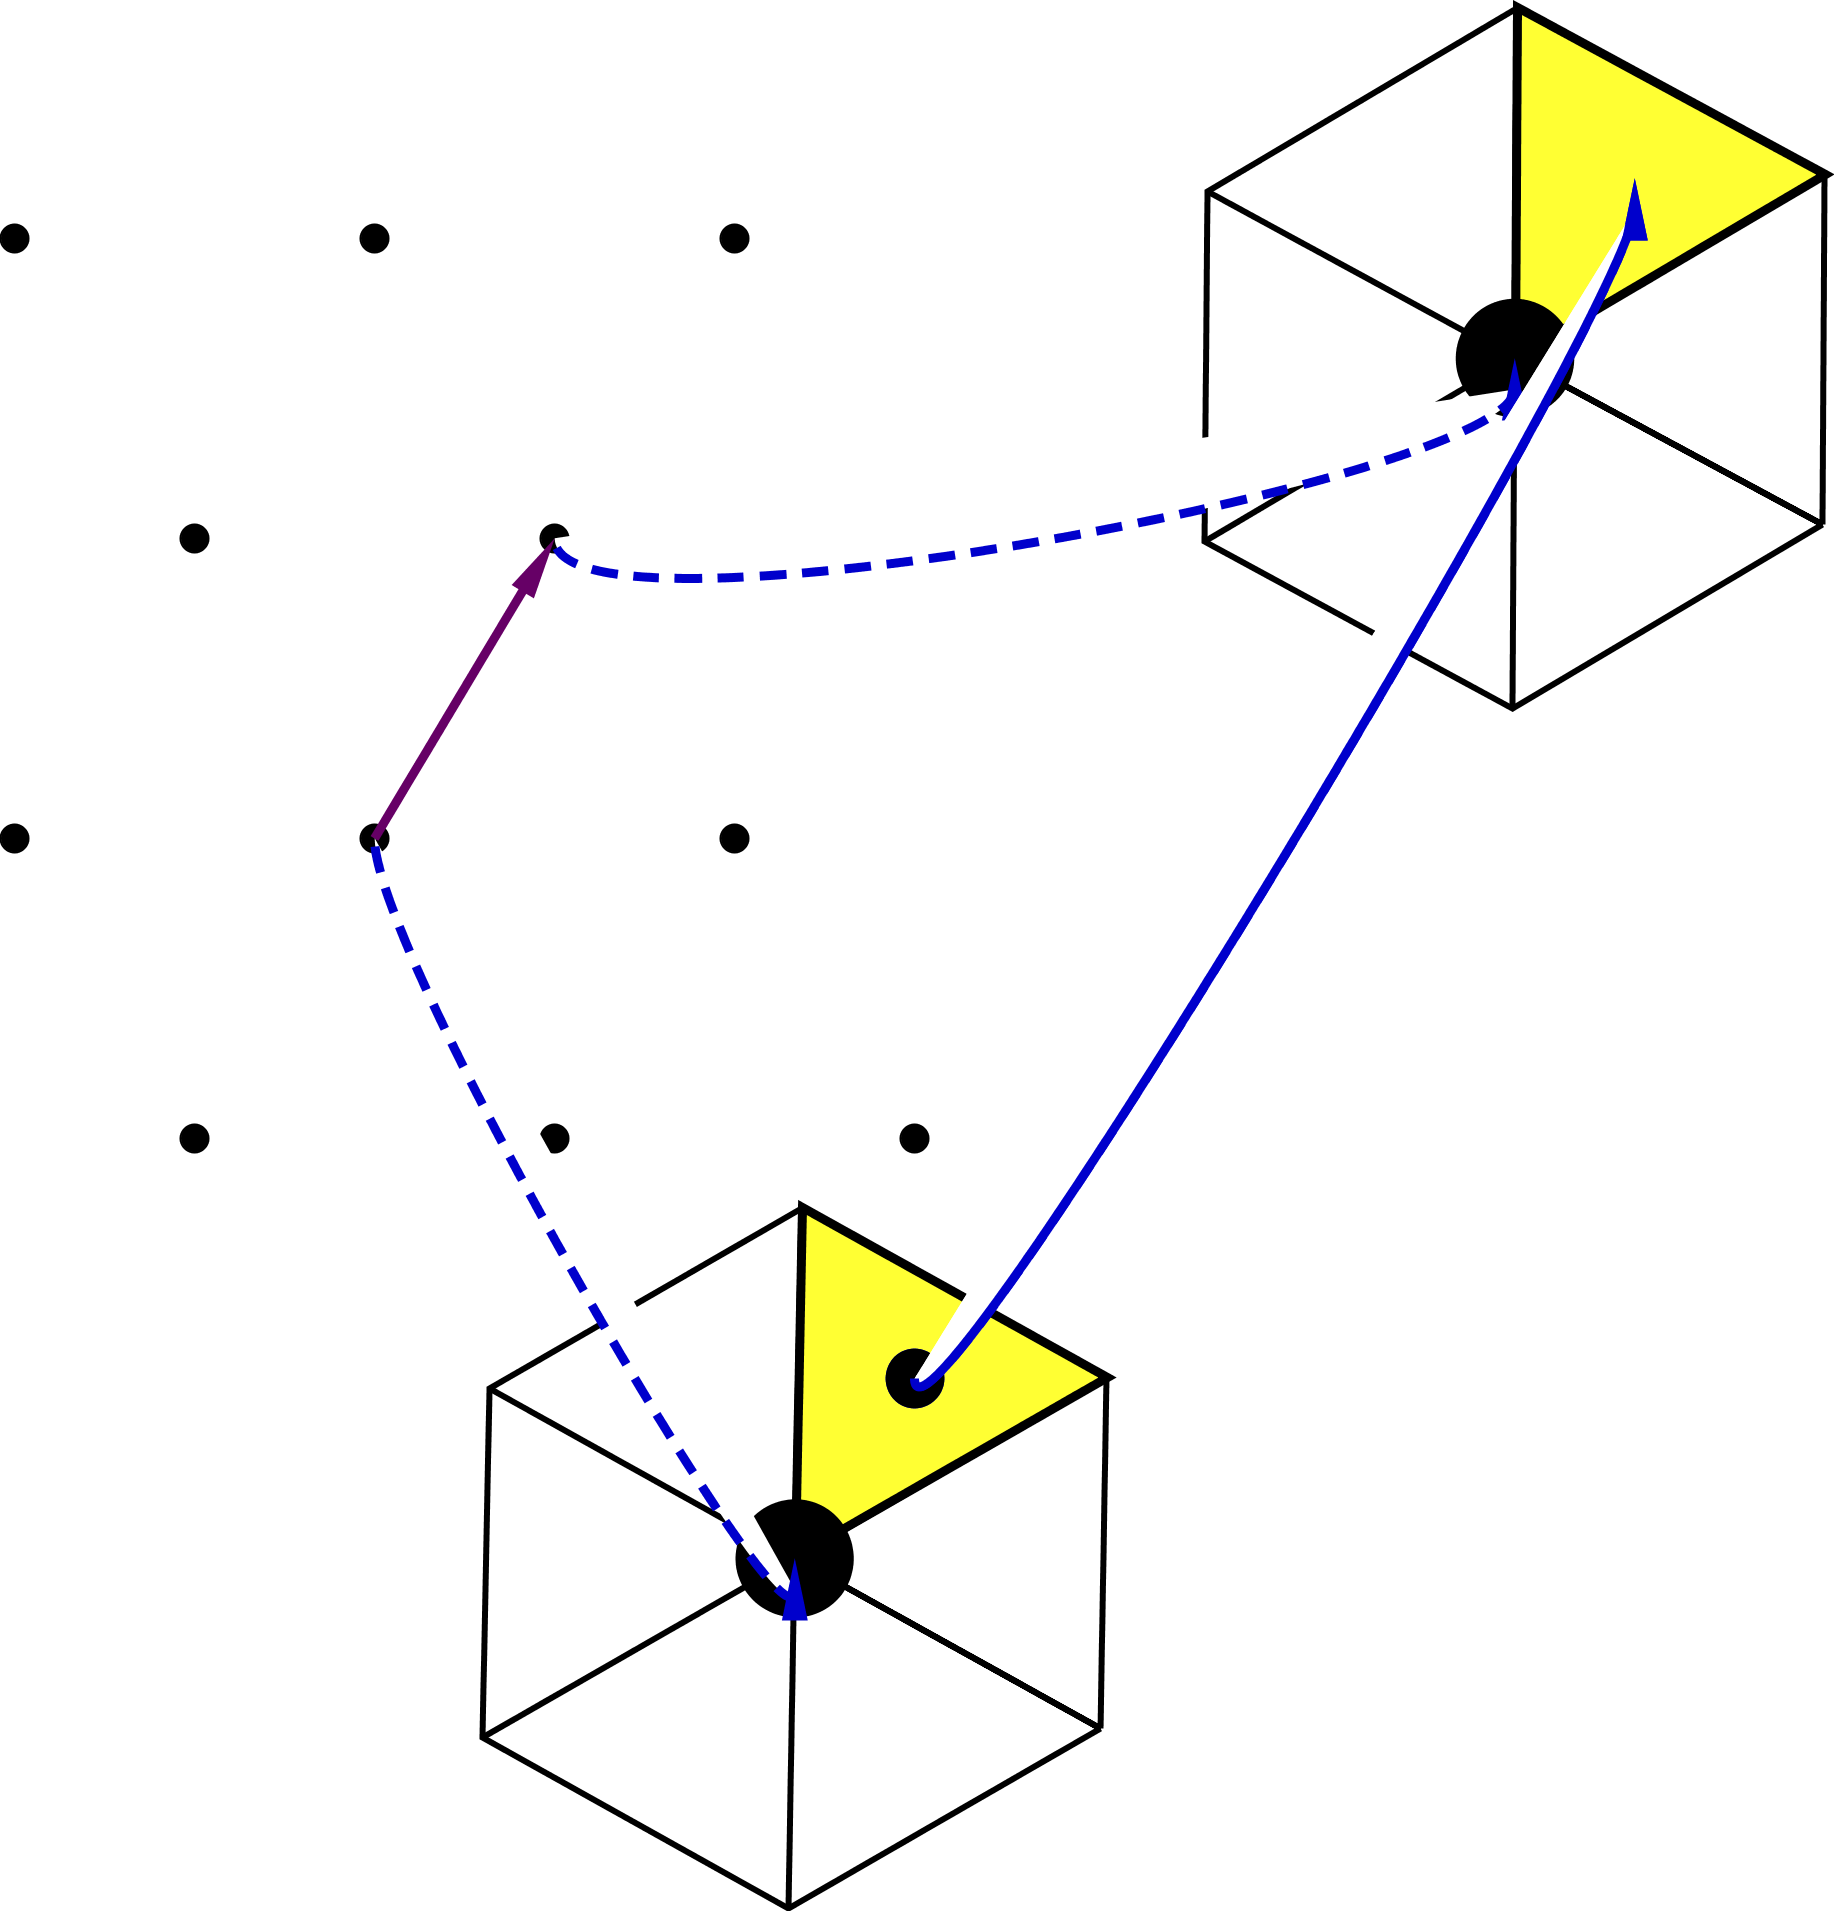
\includegraphics[width=0.7\textwidth]{./img/FHPprop}
% \caption{FHP collisions without rest particle.}
% \label{FHPprop}
%\end{figure}

%Therefore, every node consists of the six cells corresponding to these lattice vectors.
 
%Let us denote the state of the node by $\bm{n} = (n_1,n_2,n_3,n_4,n_5,n_6)$, where $n_i = 0$ stands form empty $i^{th}$ cell, and $n_i = 1$ implies that there is a particle in the $i^{th}$ cell.
% 
%We can actually identify lattice velocities of the particles with lattice vectors, as we are free to set their norm to be the same.
%
%\section{Update rule}
%In all LGCAs, the update of the lattice happens in discrete time steps and consists of two subsequent steps - collision and propagation. Both of these steps are local, so they can be treated node by node.
%
%and will be denoted by $t=1,2,3...$ and so forth. Update can be divided in two subsequent steps - collision and propagation. Both of these steps are local, so they can be treated node by node.

%The purpose of the collision is to swap as many particles in the node, as conservation of mass and momentum allows. This leads to the desirable minimization of viscosity.

%The only constraint on the collision rule is to preserve the number of particles (conservation of mass) and to preserve the total momentum in the node (conservation of momentum).

%
%Comparing it to HPP, we have a lattice with better rotational symmetry and nodes with richer  set of collisions.
%
%Now that we presented the setting of FHP in two dimensions rather intuitively, let us explore the microdynamics of FHP in a more formal way. The formal treatment provides that the hydrodynamic equations that we derive are valid for FHP in arbitrary dimension (although finding an appropriate multidimensional lattice is non-trivial and possible only in 4 dimensions, as we will see).
%
%\section{Convention that we will use}
%State of the node will be denoted by $\bm{n} = (n_1,n_2,n_3,n_4,n_5,n_6)$, where $n_i = 0$ stands for the empty $i^{th}$ cell, and $n_i = 1$ implies that there is a particle in the $i^{th}$ cell.
%
%State of a node with the position $\bf{r}$ on lattice will be denoted by $\bf{n(r)}$, whereas the state of the \textit{whole lattice} will be denoted by \textbf{n(.)}.
%
%As we know, the update happens in discrete time steps that we will denote by $t=1,2,3...$ and so forth.
%
%\section{Propagation}
%Propagation is the straight-forward step and can be captured by the simple equation
%\begin{align*}
%S n_i(\bf{r}) = n_i(\bf{r + c_i}). 
%\end{align*}
%This equation means that state of the $i^{th}$ cell in node \textbf{n(r)} \textit{propagates} along the lattice vector $c_i$ to the neighboring node $\bf{n(r + c_i)}$, the figure \ref{FHPprop}.
%
%\section{Collision}
%As we already sketched, the purpose of the collision is to swap as many particles in the node, as conservation of mass and momentum allows.
%
%For FHP in two dimensions, we have $2^6 = 64$ configurations, and whole bunch of collision configurations among them (figure \ref{FHPcol}).

%
%As we see, head-on 2-particle collisions and 4-particle collisions can result in two different states. If we wanted to preserve determinism, and we were systematically choosing only one of them, we would introduce additional, non-physical invariance - the model would become chiral. If we want to preserve the parity symmetry of the model, we need to assign equal probability to either of two final states.Hence, we are introducing non-determinism to the model.
%
%We will express the probabilities of transition from state $n$ to state $n'$ by probability matrix:
%\begin{equation}
%A(n \rightarrow n') \geq 0
%\end{equation}
%As we have 64 possible states of the node, matrix A is of dimension $64\times 64$.
%For example, the cell of matrix A that governs the head-on collisions looks like this:
%\[
% A'=
%  \begin{bmatrix}
%    0 & \frac{1}{2} & \frac{1}{2} \\
%    \frac{1}{2} & 0 & \frac{1}{2} \\
%    \frac{1}{2} & \frac{1}{2} & 0 \\
%  \end{bmatrix}
%\]
%Since the collisions are symmetric, matrix A is symmetric as well.
%
%Also, collisions are invariant to rotations or reflections of the node:
%\begin{equation}
%A(g(n) \rightarrow g(n')) = A(n \rightarrow n')
%\end{equation}
%where $g \in G$, and G is the symmetry group of the node.

%\section{Collision operator}
%Interestingly, we can express the whole update step in one simple equation using collision operator $\Delta_i$:
%\begin{equation}
%n_i(t+1,r+c_i) = n_i(t,r) + \Delta_i(t,r)
%\end{equation}
%If this equation works, then, $\Delta_i$ must be:
%\begin{enumerate}
%\item $\Delta_i = 0$ if no collision is happening in $n(t,r)$. Then state of the cell $n_i(t,r)$ only propagates to $n_i(t+1,r+c_i)$.
%\item $\Delta_i = 1$ if there is not particle in $n_i(t,r)$ yet, but gets there after collision. 
% \item $\Delta_i = -1$ if there is particle in the $n_i(t,r)$, but after collision, cell gets empty.
%\end{enumerate}
%
%\bigskip
%
%For example, $\Delta_i$ acquire very simple form for HPP:
%\begin{equation}
%\Delta_i = n_{i+1} n_{i+3}( 1 - n_i)(1 - n_{i+2}) - n_i n_{i+2}(1-n_{i+1})(1 - n_{i+3})
%\end{equation}
%As there are only 2 collision configuration in HPP, $\Delta_i$ has 2 terms.
%If either collision happens, corresponding term is 1.
%
%\section{Microscopic conservation laws}
%Using collision operator, conservation of mass and momentum is this simple:
%\begin{subequations}
%\begin{align}
%\sum_i \Delta_i(t,r) &= 0,\\
%%
%\sum_i c_i \Delta_i(t,r) &= 0
%\end{align}
%\end{subequations}
%(Prove: unfold $\Delta$s)
%Conservation laws can be equivalently expressed in the form
%\begin{align} \label{cons1}
%\begin{split}
%\sum_i n_i(t+1, r + c_i) &= \sum_i n_i(t,r), \\
%\sum_i c_i n_i(t+1, r + c_i) &= \sum_i c_i n_i(t,r).
%\end{split}
%\end{align}

